
% JuliaCon proceedings template
\documentclass{juliacon}
\setcounter{page}{1}

\usepackage{caption}
\usepackage{booktabs,siunitx}
\usepackage{outlines}
\usepackage[xindy, acronym, nopostdot, style = super, nonumberlist, toc, nomain]{glossaries}
% -----------------  B  ----------------
\newacronym{bea}{BEA}{Bureau of Economic Analysis}

% -----------------  C  ----------------
\newacronym{cbsa}{CBSA}{core-based statistical area}
\newacronym{cge}{CGE}{computable general equilibrium}
\newacronym{cfs}{CFS}{Commodity Flow Survey}
\newacronym{csa}{CSA}{combined statistical area}

% -----------------  E  ----------------
\newacronym{eia}{EIA}{Energy Information Administration}

% -----------------  G  ----------------
\newacronym{gams}{GAMS}{General Algebraic Modeling System}
\newacronym{gsp}{GSP}{Gross State Product}
\newacronym{gtap}{GTAP}{Global Trade Analysis Project}

% -----------------  M  ----------------
\newacronym{mpsge}{MPSGE}{Mathematical Programming System for General Equilibrium}

% -----------------  N  ----------------
\newacronym{naics}{NAICS}{North American Industry Classification System}
\newacronym{nass}{NASS}{National Agricultural Statistics Service}
\newacronym{nrel}{NREL}{National Renewable Energy Laboratory}

% -----------------  P  ----------------
\newacronym{pce}{PCE}{Personal Consumer Expenditures}
\newacronym{pep}{PEP}{Process Economics Program}

% -----------------  R  ----------------
\newacronym{reeds}{ReEDS}{Regional Energy Deployment System}

% -----------------  S  ----------------
\newacronym{scea}{SCEA}{Scientific Computing and Energy Analysis}
\newacronym{sctg}{SCTG}{Standard Classification of Transported Goods}
\newacronym{seds}{SEDS}{State Energy Data System}
\newacronym{slug}{SLUG}{SLiDE User Group}
\newacronym{sgf}{SGF}{State Government Finance}
\newacronym{siip}{SIIP}{Scalable Integrated Infrastructure Planning}
\newacronym{slide}{SLiDE}{Scalable Linked Dynamic Equilibrium}

% -----------------  T  ----------------
\newacronym{tempo}{TEMPO}{Transportation Energy \& Mobility Pathway Options}

% -----------------  U  ----------------
\newacronym{us}{U.S.}{United States}
\newacronym{usgs}{USGS}{United States Geological Survey}
\newacronym{usrep}{USREP}{U.S. Regional Energy Policy}

% -----------------  W  ----------------
\newacronym{windc}{WiNDC}{Wisconsin National Data Consortium}

\captionsetup{width=0.9\textwidth}

\begin{document}

% **************GENERATED FILE, DO NOT EDIT**************

\title{Intertwined Economic and Energy Analysis\\using Julia}

\author[1]{Caroline Lockhart Hughes}
\author[1]{Maxwell Brown}
\affil[1]{National Renewable Energy Laboratory}

\keywords{Julia, Optimization, Game theory, Compiler}

\hypersetup{
pdftitle = {Intertwined Economic and Energy Analysis using Julia},
pdfsubject = {JuliaCon 2020 Proceedings},
pdfauthor = {Caroline Lockhart Hughes, Maxwell Brown},
pdfkeywords = {Julia, computable general equilibrium},
}

\maketitle

% This talk introduces the SLiDE.jl package, which leverages U.S. economic data to assess economic implications of energy infrastructure planning to answer these and other questions.
% The Scalable Linked Dynamic Equilibrium (SLiDE) model is an implementation of a computable general equilibrium (CGE) model. CGE models are commonly used for detailed regional economic analysis of inputs, outputs, prices and quantities of various economic sectors to inform policy decisions. This talk will focus on the development of the data management approach with a focus on usability.

% We will delve into the inner workings of the SLiDE module to explore the benefits and challenges of using Julia for data science applications. Techniques used to standardize the publicly available blueNOTE dataset include autogenerated and populated structs and powerful multiple dispatch and methods. Discussion will include the design-thinking approach taken to create a user-friendly interface to scale the model in space, time, and sector and encourage further adoption of Julia in policy analysis.

\begin{abstract}
Energy and the economy are deeply intertwined yet the models typically employed for energy analysis treat the energy sector in isolation while lacking the capability to robustly represent the \gls{us} economy.
The \href{http://github.com/NREL/SLiDE}{SLiDE.jl} package package leverages \gls{us} economic data to assess economic implications of energy infrastructure planning to answer these and other questions.
\end{abstract}

\section{Introduction}

The \gls{slide} model aims to remove the overly-simplistic and static assumptions concerning economic boundary conditions by developing a model of the economy and coupling that model with detailed, engineering-focused energy system models.
\gls{slide} is part of the \gls{siip} framework, which is an initiative housed under \gls{nrel}'s \gls{scea} directorate to unify models under one umbrella.
Other \gls{siip} models include
% \gls{reeds}, \dots; and
% \gls{tempo}, \dots.

% \gls{slide}

\section{Methodology}
\gls{slide} builds on foundational work by the \gls{windc} \cite{rutherford-2019:tools}.
\gls{windc} compiled the blueNOTE dataset, which is comprised of data made available from the 

The original dataset is generated in Python and is used in a \gls{cge} model implemented in \gls{gams} \cite{brooke-1988:gams}.

\section{Data Processing}

Before the input data can be used, it must be cleaned and standardized.
The \gls{slide} package includes data processing capabilities that promote clarity when handling multiple files and enable simple operation definition.

\gls{slide} relies on data that are updated between monthly, in the case of \gls{us} Trade Data, to every five years, in the case of \gls{cfs} data.
On occasion, when historical data is revised, the required edits are subject to change.
In this case, it is important to have a user-friendly method to make necessary updates quickly.

Data operations are stored in yaml files to promote readability.


% \begin{loutline}[enumerate]
% \1 Define
% \end{loutline}

% Model validation
This standardized data processing approach aides model validation by creating a clear record of how each input data file was edited.

% \section{Example}

% \ref{tab:nass-in} shows a portion of unedited \gls{nass} data.
% \ref{tab:nass-out} shows it has been cleaned to be used in the \gls{slide} model.
% This section describes the process the user undertakes to define these edits, as well as the internal process taken to apply these changes.

\section{User-Centered Data Editing}
The \gls{slide} data processing is designed to be user-friendly to encourage new adoption of both Julia and the \gls{slide} \gls{cge} model.
% \subsection{User Interfacing Code}
All of the necessary edits are defined in a yaml file.
Users have the option to defined all of their edits in individual yaml files or to write yaml files in spreadsheet columns%
%, as shown in \ref{fig:generate-yaml.png}
.
In case there are a large number of files to edit, defining edits in a place where it is easy to scan over all of the possible edits will reduce the cognitive load the user must take on when defining these edits, thus reducing the time spent writing and revising these files when needed.
This approach also helps ensure consistency across the edits made to all files.

\begin{outline}[enumerate]
\1 Write yaml files as spreadsheet columns.
This enables easier scanning across yaml files and their associated edits so that users can keep track of the edits they've made.
\1 \texttt{write\_yaml()} will write a yaml file containing the information in each spreadsheet column.
\1 \texttt{run\_yaml} will:
\2 Read the input file.
\2 Make the user-defined edits.
\2 Write the resulting data file in the specified \texttt{``PathOut''}.
\end{outline}

% \subsection{Editing structures}
% Each \gls{slide}-enabled data edit is stored in its own \texttt{struct}.
% Possible edits include:

% \gls{slide.jl}

\section*{Acknowledgments}
We acknowledge the \glsentryfull{windc} for laying the groundwork for \gls{slide}.
In particular, we would like to thank Thomas Rutherford, Adam Christensen, and Andrew Schreiber, and G\:ok\,ce Akin-Ol\,cum for their work with the blueNOTE dataset and \gls{windc}-based \gls{cge} model.

\begin{figure*}
    \centering
    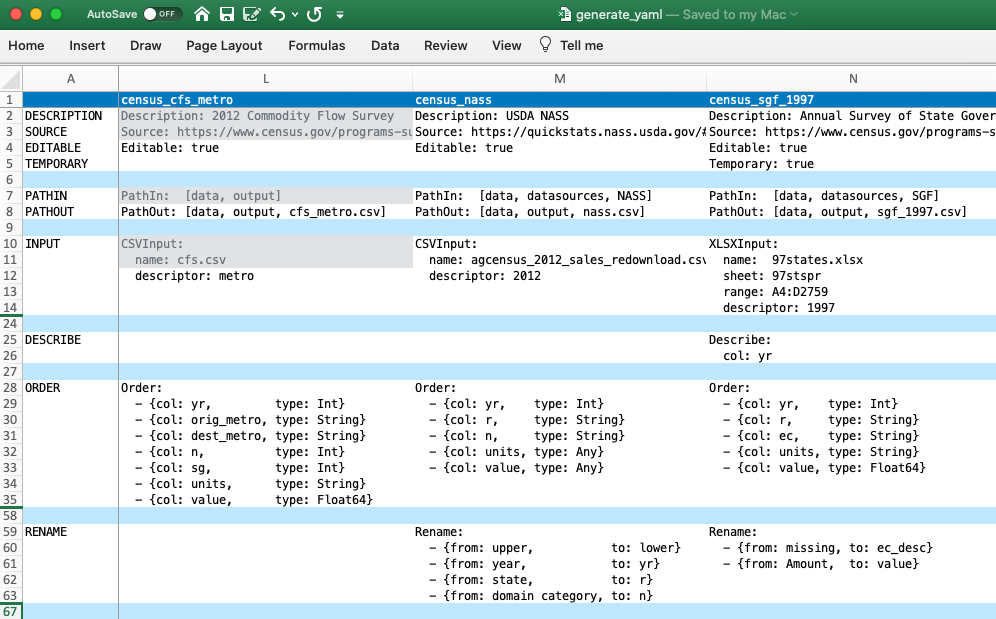
\includegraphics[width = \textwidth]{fig/excel-yaml.png}
    \caption{Spreadsheet with defined data process}
    \label{fig:excel-yaml}
\end{figure*}

\begin{table*}[t]
\begin{minipage}{\textwidth}
\centering
\caption{Unedited \gls{nass} data.}
\resizebox{\textwidth}{!}{%
\begin{tabular}{llllllllll}
\toprule
Program & Year & Period & Week Ending & Geo Level & State &\dots& Domain Category & Value & CV (\%) \\\midrule
CENSUS & 2012 & YEAR & & STATE & WISCONSIN && NAICS CLASSIFICATION: (111)    & 3,759,611,000 & 0.9 \\
CENSUS & 2012 & YEAR & & STATE & WISCONSIN && NAICS CLASSIFICATION: (1111)   & 2,656,140,000 & 1.1 \\
CENSUS & 2012 & YEAR & & STATE & WISCONSIN && NAICS CLASSIFICATION: (11111)  & 166,698,000   & 2.3 \\
CENSUS & 2012 & YEAR & & STATE & WISCONSIN && NAICS CLASSIFICATION: (11112)  & (D)           & (D) \\
\bottomrule
\end{tabular}
}
\label{tab:nass-in}

\bigskip
\caption{\gls{nass} data edited in preparation for use in the model.}
\begin{tabular}{llllS[table-format=4.3]}
\toprule
yr   & r  & n     & units                        & {value}    \\\midrule
2012 & wi & 111   & millions of us dollars (USD) & 3759.611 \\
2012 & wi & 1111  & millions of us dollars (USD) & 2656.14  \\
2012 & wi & 11111 & millions of us dollars (USD) & 166.698  \\
2012 & wi & 11112 & millions of us dollars (USD) & 0.0      \\
\bottomrule
\end{tabular}
\label{tab:nass-out}
\end{minipage}
\end{table*}

% **************GENERATED FILE, DO NOT EDIT**************

\bibliographystyle{juliacon}
\bibliography{ref.bib}

\end{document}

% Inspired by the International Journal of Computer Applications template